\chapter{Kravspecifikation}

\begin{longtabu} to \linewidth{@{}l l l X[j]@{}}
    Version &    Dato &    Ansvarlig &    Beskrivelse\\[-1ex]
    \midrule
    0.1 &	8/09 2015	&	Alle		& Oprettelse  af dokument\\
    0.2 &	21/09 2015 & 	Alle		& Første udkast til kravspecifikation og use cases\\
    0.3 &	24/09 2015 & Alle 	& Fully-dressed use cases\\
    0.5 &	30/09 2015 & Alle 	& Udarbejdelse af ikke-funktionelle krav\\
    0.6  & 07/10 2015 & Alle 	& Kravspecifikation rettelser efter review\\ 
    1.0 & 	04/11 2015 & TSN, JTH, MFJ & Nye fully-dressed use cases, mere software relaterede\\   
\label{version krav}
\end{longtabu}


\section{Indledning}
 Et blodtryksmålingssystem er blevet udarbejdet, der helt generelt er opbygget af en hardware-del og en software-del. Hardware-delen er opbygget af en forstærker, transducer og analogt filter hvis formål er at kunne forstærke og filtrere blodtrykssignalet og software-delen kalibrerer, nulpunktsjusterer og analyserer signalet, samt viser signalet grafisk på en brugergrænsefalde. \\[1ex]
 Kravspecifikationen beskriver produktets kunnen ud fra opstillede funktionelle og ikke-funktionelle krav til systemet. De ikke-funktionelle krav er krav, der er opstillet til selve systemet, og de funktionelle krav er beskrevet i use cases, som omhandler systemets aktiviteter i forhold til aktører og mål. 


\section{Funktionelle krav}
\subsection{Aktør-kontekst diagram}

\begin{figure}[H]
	\centering
	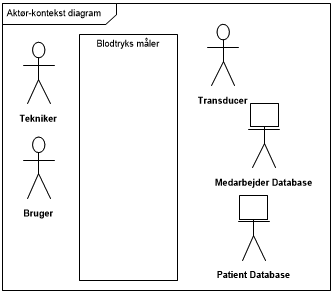
\includegraphics[width=0.5\textwidth]{Figurer/ISE/aktdiagram2}
	\caption{Aktør-kontekst diagram}
	\label{Aktdiagram}
\end{figure}


\subsection{Aktørbeskrivelse}

\begin{longtabu}to \linewidth{@{}l l X[j]@{}}
	{\large \textbf{Aktørnavn}} & {\large \textbf{Type}} & {\large \textbf{Beskrivelse}}\\ \toprule
	Bruger & Primær & Brugeren er den aktør, der foretager blodtryksmålingerne. Brugeren er en person, der har kendskab til systemet, samt tilladelse til at benytte systemet. F.eks. en læge eller anæstesisygeplejerske \\
	Tekniker & Primær & Tekniker er den aktør, der foretager den årlige kalibrering af systemet. Teknikeren er en person, der har kendskab til den tekniske del af systemet. F.eks. en medicotekniker på et sygehus\\
	Transducer & Sekundær & Transducere omformer blodtryk til et elektrisk signal\\
	Medarbejder database & Sekundær & Medarbejder-databasen er det sted, hvor medarbejderens login valideres \\
	Patient-database & Sekundær & Patient-databasen er det sted, hvor blodtryksmålingens data gemmes og patientens CPR-nummer valideres \\ \bottomrule
\caption{Aktørbeskrivelse}
\label{Aktoerbeskrivelse}
\end{longtabu}

\section{Use cases}
\subsection{Use case diagram}
\begin{figure}[H]
	\centering
	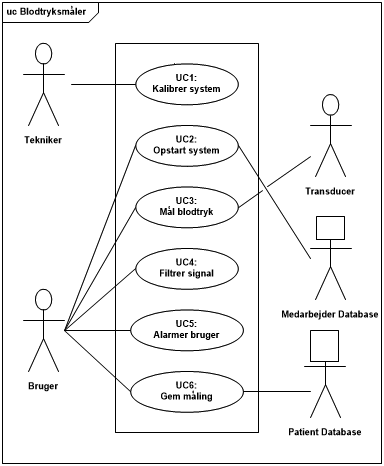
\includegraphics[width=0.7\textwidth]{Figurer/ISE/UcDiagram2}
	\caption{Use case diagram}
	\label{UC diagram}
\end{figure}

\subsection{Use case 1}

\begin{longtabu} to \linewidth{@{}l r X[j]@{}} %UC1%
    {\large \textbf{Use case 1}} && \\
    \toprule
    Navn &&    Kalibrer system\\
    Use case ID &&    1\\
    Samtidige forløb &&    1\\
    Primær aktør &&    Tekniker\\
    Initialisere &&    Tekniker\\
    Mål && Tekniker ønsker at foretage kalibrering\\
    Forudsætninger &&  Tekniker har adgang til systemet\\
    Resultat &&    Systemet er kalibreret                     \\ \midrule
    Hovedforløb &    1. &    Tekniker måler og noterer atmosfærisk tryk \\
    			&    2. &    Tekniker påtrykker systemet tre kendte tryk  \\
    			&    3. &    Tekniker aflæser responserne  \\ 
    			&    4. &    Tekniker noterer afvigelser fra de kendte tryk \newline [\textit{4.a Der er ingen afvigelser}]  \\
    			&    5. &    Tekniker kalibrerer i forhold til afvigelsen  \\ \midrule 		
    Undtagelser &    4.a & Use case afsluttes \\ \bottomrule
\caption{Fully-dressed use case 1}
\label{UC1}
\end{longtabu}

\subsection{Use case 2}

\begin{longtabu} to \linewidth{@{}l r X[j]@{}} %UC2%
    {\large \textbf{Use case 2}} && \\
    \toprule
    Navn &&    Opstart system\\
    Use case ID &&    2\\
    Samtidige forløb &&    1\\
    Primær aktør &&    Brugeren\\
    Sekundær aktør && Medarbejder-database\\
    Initialisere &&    Brugeren\\
    Mål && Systemet er opstartet\\
    Forudsætninger &&  Forbindelse til database\\
    Resultat &&    Systemet er nulpunktsjusteret og brugeren er klar til at blive forbundet til systemet\\
    \midrule
    Hovedforløb &   1. & Brugeren indstiller transduceren til at måle det atmosfæriske tryk\\ 
    	&			2. & Brugeren trykker på "nulstil"\--knappen. Systemet laver nulpunktsjustering \\ 
    	& 			3. & Brugeren indstiller transduceren til at måle blodtryk\\
    	&			4. &    Brugeren indtaster login-oplysninger og trykker på "Log ind"\--knappen. Systemet tjekker i databasen om oplysninger er gyldige \newline [4.a \textit{Forkert login}]\\
    	\midrule
    Undtagelser &    4a. & Besked om forkert login vises. Use case fortsættes fra punkt 4     \\ \bottomrule    
\caption{Fully-dressed use case 2}
\label{UC2}
\end{longtabu}

\subsection{Use case 3}

\begin{longtabu} to \linewidth{@{}l r X[j]@{}} %UC3%
    {\large \textbf{Use case 3}} && \\
    \toprule
    Navn &&    Mål blodtryk\\
    Use case ID &&    3\\
    Samtidige forløb &&    1\\
    Primær aktør &&    Brugeren\\
    Initialisere &&    Brugeren\\
    Mål && Blodtryksmåling er igangsat\\
    Forudsætninger && UC2 er gennemført\\
    Resultat &&    Blodtrykket vises kontinuerligt i en graf. Puls, systoliske og diastoliske værdier vises i blodtryksvinduet                 \\ \midrule
    Hovedforløb &    1. &    Brugeren trykker på "Start"\--knappen i blodtryksvindue\\
    			& 	 2. & Transduceren måler blodtryk\\
    			&	 3. & Systemet modtager blodtryksmåling fra transduceren\\
    			& 	 4. & Blodtrykgraf, systolisk, diastolisk og puls vises grafisk i blodtryksvinduet\\  \bottomrule
\caption{Fully-dressed use case 3}
\label{UC3}
\end{longtabu}

\subsection{Use case 4}

\begin{longtabu} to \linewidth{@{}l r X[j]@{}} %UC4%
    {\large \textbf{Use case 4}} && \\
    \toprule
    Navn &&    Filtrer signal\\
    Use case ID &&    4\\
    Samtidige forløb &&    2\\
    Primær aktør &&    Brugeren\\
    Initialisere &&    Brugeren\\
    Mål && Der kan foretages en digital filtrering af signalet\\
    Forudsætninger && UC3 er gennemført\\
    Resultat &&    Det filtrerede signal vises i blodtryksgrafen                    \\ \midrule
    Hovedforløb &    1. &    Brugeren trykker på "Til"\--knappen under filter\\
    			&	 2. & 	 Systemet filtrerer signalet\\
    			&	 3. 	&	 Det filtrerede signal vises i blodtryksvindue \\ \bottomrule               
\caption{Fully-dressed use case 4}
\label{UC4}
\end{longtabu}

\subsection{Use case 5}

\begin{longtabu} to \linewidth{@{}l r X[j]@{}} %UC5%
    {\large \textbf{Use case 5}} && \\
    \toprule
    Navn &&    Alarmer bruger\\
    Use case ID &&    5\\
    Samtidige forløb &&    2\\
    Primær aktør &&    Brugeren\\
    Initialisere &&   Brugeren\\
    Mål && Systemet kan alarmere bruger ved for højt/lavt blodtryk\\
    Forudsætninger && UC3 er gennemført\\
    Resultat &&    Systemet alarmerer bruger                    \\ \midrule
    Hovedforløb &    1. &    Brugeren tilpasser diastoliske og systoliske grænseværdier ud fra patientens normale blodtryk\\ 
    			& 	 2. & 	Systemet tjekker om grænseværdier er overskredet\\ 
    			&	 3. & 	Målte blodtryk overskrider valgte grænseværdier\newline [\textit{3.a Målte blodtryk overskrider ikke valgte grænseværdier}]\\ 
    			& 	 4. & 	Alarm startes \newline [\textit{4.a Bruger udskyder alarm}]\\ \midrule            
    Undtagelser &    3.a & Use case fortsættes fra punkt 2 \\ 
    			&	 4.a & Alarm udskydes med 3 minutter, og use case startes fra punkt 2 igen\\ \bottomrule
\caption{Fully-dressed use case 5}
\label{UC5}
\end{longtabu}

\subsection{Use case 6}

\begin{longtabu} to \linewidth{@{}l r X[j]@{}} %UC6%
    {\large \textbf{Use case 6}} && \\
    \toprule
    Navn &&    Gem måling\\
    Use case ID &&    6\\
    Samtidige forløb &&    1\\
    Primær aktør &&    Brugeren\\
    Mål &&    Brugeren ønsker at afslutte systemet og gemme måling\\
    Forudsætninger && UC3 er gennemført\\
    Resultat &&    Blodtryksmålingens data er gemt i database, og bruger er logget ud af systemet                    \\ \midrule
    Hovedforløb &    1. &    Brugeren trykker på "Afslut"\--knappen. "Gem"\--vindue åbnes. \newline [1.a \textit{Bruger ønsker ikke at afslutte}]\\  						 	
                &    2. & Brugeren indtaster CPR-nummer og trykker på "Gem"\--knappen \newline [2.a \textit{CPR-nummer er ikke gyldigt}]\\
                &    3. & Besked om at data er gemt vises. Brugeren trykker på "Ok"\--knappen. Systemet logger ud, og use case 2 startes
                	\\ \midrule                
    Undtagelser &    1.a. & Bruger trykker på "Annuller"\--knappen. Systemet lukker "Gem"\--vinduet ned\\ 
    			&	2.a. &  Besked om at CPR-nummer ikke er gyldigt, vises. Nyt CPR-nummer indtastet. Use case fortsættes fra punkt 2\\ \bottomrule
    		
\caption{Fully-dressed use case 6}
\label{UC6}
\end{longtabu}

\section{Ikke-funktionelle krav}
\subsection{(F)URPS+}
MoSCoW er angivet i parentes ved hhv. M, S, C og/eller W, for Must, Should, Could og Won't\\


\textbf{Functionality}\\
\begin{enumerate}
	\item (M) Brugeren skal kunne starte en ny måling inden for 30 sekunder efter opstart af programmet \\
	\item (M) Systemet skal kunne forstærke signalet fra transduceren 400 gange\\
	\item (M) Systemet skal kunne filtrere signalet med det indbyggede analoge filter med en båndbredde på 50Hz, samt en cut-off frekvens ved 50Hz \\
	\item (M) Programmet skal kunne vise blodtrykssignalet kontinuert\\
	\item (M) Programmet skal programmeres i C\#\\
	\item (M) Programmet skal kunne lagre de målte data i en database\\
	\item (M) Systemet skal kalibreres årligt\\
	\item (S) Programmet bør kunne måle puls\\
\end{enumerate}

\textbf{Usability}\\
\begin{enumerate}
	\item (M) Blodtrykstallene der udskrives på brugergrænsefladen er røde\\
	\item (S) Pulsmålingen bør udskrives på brugergrænsefladen med grønne tal\\
	\item (M) Brugergrænsefladen skal leve op til figuren udarbejdet i designafsnittet, se afsnit \ref{GUI} \\
\end{enumerate}

\textbf{Reliability}\\
\begin{enumerate}
	\item (M) Systemet skal kunne køre uden fejl i et år\\
	\item (M) Systemet skal have en ”mean time to restore” på højest 24 timer\\
	\subitem Systemet får herved en tilgængelighed beregnet ved \begin{align}
Availability = \frac{MTBF}{MTBF+MTTR} = \frac{365}{365+1} = 0,997 = 99,7\%
\end{align}\\
\end{enumerate}

\textbf{Performance}\\
\begin{enumerate}
	\item (S) Systemet bør kunne gemme data på 5 sekunder +/-10\%\\
\end{enumerate}

\textbf{Supportability}\\
\begin{enumerate}
	\item (M) Softwaren skal opbygges efter trelagsmodellen\\
\end{enumerate}




















